% brainstorm:

% * revisão das teorias de contornos
% * parte da análise que fiz do opus 5 mov 3 de Webern
% * exemplos de usos de operações na peça do mestrado e experimentos
% * desenvolvimento do goiaba (para que serve e um exemplo da saída)

\section{Introduction}
\label{sec:introduction}
Contour is the shape or format of objects. In Music, they can be
associated to elements like pitch, density, rhythm, and can represent
a parameter in function of another, such as pitch in function of time.
The contour of musical excerpts can be easily recognized from a
graphic representation by professionals and laymen alike
\cite{marvin88:generalized}. For instance, Beethoven's Fifth
Symphony's main motive and its pitch contour are represented
respectively in figures \ref{fig:5a-sinfonia-motivo} and
\ref{fig:c-3120}.

Technically, a contour is an ordered set of numbered elements
\cite{morris93:directions}. Absolute values of contour elements are
ignored, and only the high-low relationship between them is
regarded. For instance, figures \ref{fig:5a-sinfonia-motivo} and
\ref{fig:ly-3120} have the same pitch contour, graphically represented
in figure \ref{fig:c-3120}, and symbolically by F(3 1 2 0). The
uppercase letter names the contour.

The study of Contour is important because, like motives and pitch
sets, contours help to give coherence to a composition. They are
structural devices that can be combined through operations like
inversion and retrogradation, and can be approached by analytical or
compositional points of view.

Systematic study about the usage of contour in musical composition are
scarce, despite the possible coherence that contours can give and the
rich operations provided by contour theories (see section
\ref{sec:contour-theories}). Besides, contour operations need precise
mathematical calculations and their graphical representations use
plotting intensely. For these reasons a computer program to calculate
and plot contours and its operations may be of great value for the
composer wanting to use contours in his or her compositions. We
believe that the formal use of contours in the field of composition
needs more experimentation and study. In this paper we present the
partial results of our research\footnote{Additional information was
  omitted to keep anonymity and will be included in final version.} on
the use of contour in musical compositions. We are developing a
contour processing software that receives as input symbolic contours
and outputs symbolic and graphical representations of contours and its
operations. Also, the first author of this paper, in his master's
research, composed a woodwind quintet based in contour theories
operations using the mentioned software (see section
\ref{sec:contour-composition}).

\section{Contour theories}
\label{sec:contour-theories}

Many authors
\cite{friedmann85:methodology,friedmann87:response,morris87:composition,morris93:directions,marvin.ea87:relating,marvin88:generalized,marvin.ea95:generalization,polansky.ea92:possible,quinn97:fuzzy,clifford95:contour,beard03:contour}
have developed theories to organize systematically the knowledge about
contour. These theories were developed primarily as analytic
techniques for non-tonal compositions \cite{beard03:contour}, and
provide arrays, matrices and many operations to help the comparison of
contours, like inversion, translation, comparison matrix, and contour
interval array.

Music analysis under the point of view of contour have been effective
in tonal and non-tonal music. There are successful analysis of pieces
by A. Schoenberg \cite{friedmann85:methodology}, A. Webern
\cite{clifford95:contour}, L. Dallapicolla
\cite{marvin88:generalized}, and W. A. Mozart \cite{beard03:contour}
pieces. Clifford \cite{clifford95:contour}, for example, says contour
has a significant role in Webern pre-serial music structure.

\section{The usage of contour in Composition}
\label{sec:contour-composition}

The quintet mentioned in section \ref{sec:introduction} was composed
entirely using the contour processor software to simplify operations
and plotting. The piece is based on combinations of contour operations
associated to parameters such as pitch, tempo, density and texture.
This quintet is based on a six notes motive ($\alpha$, seen in fig.
\ref{fig:motivo-alfa}) and its derived contour P(5 3 4 1 2 0) (fig.
\ref{fig:c-534120}). Only this contour P, its subsets and
operations---retrogradation, inversion, rotation, interpolation---were
used in the piece.

For instance, the tempos in this quintet---82, 66, 120, 108 and
112---have relations based in the contour A(1 0 4 2 3), a subset of P.
The number of instruments in the first section, N(1 3 2 5 4), are also
based in a subset of contour P. The piece begins with a solo, then a
trio, a duo, a quintet, and finally a quartet.

Contour operations were also combined to produce new material.
Rotation was combined with retrogradation, intervalic expansion with
interpolation, rotation with intervalic expansion, and so on.

The contour software was essential to compose a \eng{fugato}, in the
quintet, because each piece of subject and counter-subject were based
on different combinations of rotation and retrogradation operations.
The subject has the original contour P(5 3 4 1 2 0) and rotation with
a factor 3 (fig. \ref{fig:sujeito-fugato}). The graphical
representations of these subject operations as outputed by the contour
software can be seen in figure \ref{fig:output-sujeito-fugato}. The
counter-subject has the retrogradation of the original contour repeated
three times with different rotation factors---5, 4 and 3 (fig.
\ref{fig:contra-sujeito-fugato}). The output of the software for these
operations are in figure \ref{fig:output-contra-sujeito-fugato}.

Rotation and intervalic expansion occur like in figure
\ref{fig:notas-curtas-madeiras}. In the flute the contour has its
original form, and in the clarinet there is a rotation with a factor 2
and an expansion. In the oboe there is a rotation with a factor 3 and
contour deviation justified by the gesture. In the bassoon there is a
factor 3 contour rotation and retrogradation, and intervalic
expansion.

\section{Conclusions}
\label{sec:conclusions}

Contour was a significant structural device in the cited quintet
compositional process. The majority structures of the piece were
composed based on contour operations. For this reason we believe
contour is as important to composition as to analysis.

The cited software has an important role in our research, automating
operations calculation and plotting. It can be very useful for
composition and analysis. In the future the software will also receive
as input scores in the Lilypond\footnote{\url{http://lilypond.org/}}
format and will have a graphical interface. The next step in our
research is to develop the software to provide a better interaction
with the user, and to compose short experiments. The aim of these
experiments is to test more operations and multiple layer contours,
like simultaneous association with pitch, duration, timbre and
dynamics.

\break
%%% concentra figuras em um só lugar

\begin{figure}[!p]
  \centering
  \subfloat[Main motive]{
    \includegraphics{5a-sinfonia}
    \label{fig:5a-sinfonia-motivo}
  }
  \subfloat[Contour F(3 1 2 0)]{
    \includegraphics{c-3120}
    \label{fig:c-3120}
  }
  \caption{The Fifth Symphony's main motive and its melodic contour}
  \label{fig:5a-sinfonia}
\end{figure}

\begin{figure}
  \centering
  \includegraphics{ly-3120-qualquer}
  \caption{A melody with F(3 1 2 0) contour}
  \label{fig:ly-3120}
\end{figure}

\begin{figure}[!p]
  \centering
  \subfloat[$\alpha$ motive]{
    \includegraphics{motivo-alfa}
    \label{fig:motivo-alfa}
  }
  \subfloat[P(5 3 4 1 2 0) contour]{
    \includegraphics{c-534120}
    \label{fig:c-534120}
  }
  \caption{Materials}
  \label{fig:materials}
\end{figure}

\begin{figure}
  \centering
  \subfloat[Subject]{
    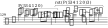
\includegraphics[scale=3.2]{sujeito-fugato}
    \label{fig:sujeito-fugato}
  }

  \subfloat[Counter-subject]{
    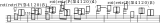
\includegraphics[scale=3.2]{contra-sujeito-fugato}
    \label{fig:contra-sujeito-fugato}
  }
  \caption{Structural elements of \eng{fugato}}
  \label{fig:elementos-fugato}
\end{figure}

\begin{figure}
  \centering
  \subfloat[Subject]{
    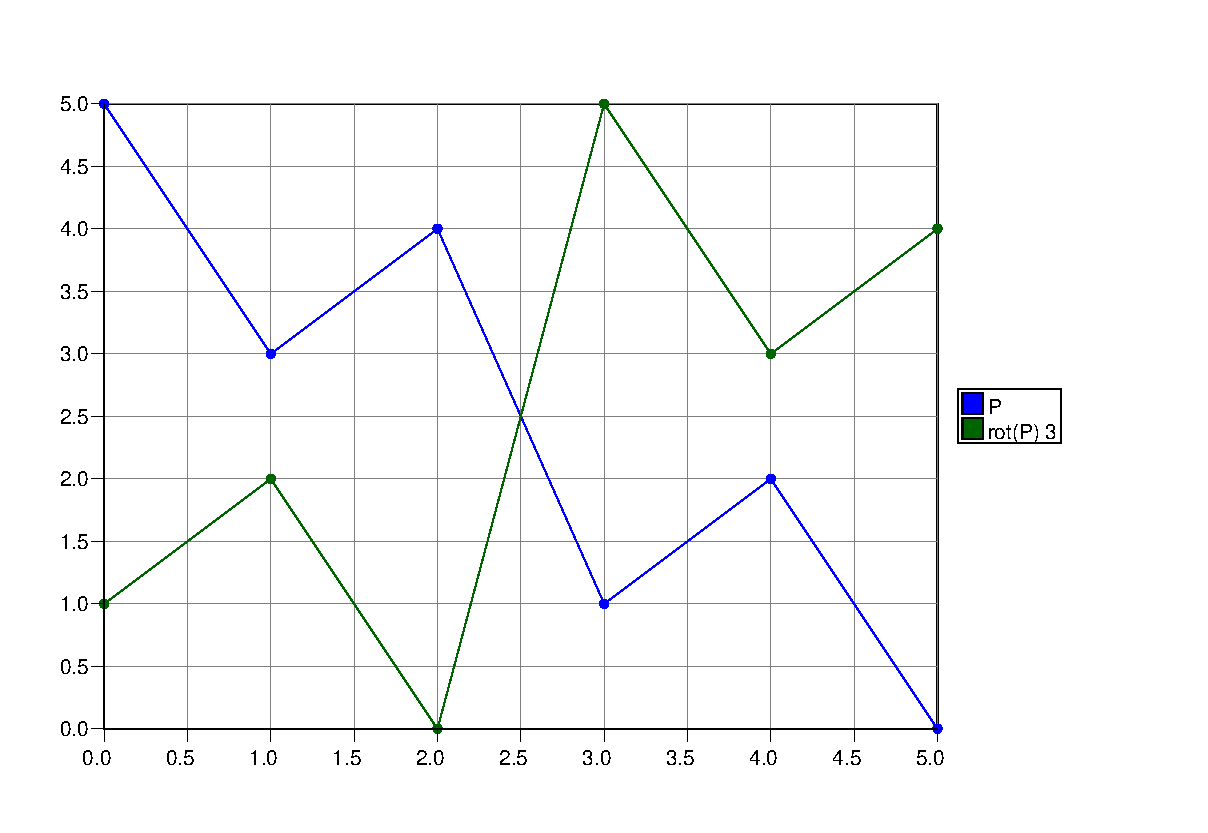
\includegraphics[scale=.44]{output-subject}
    \label{fig:output-sujeito-fugato}
  }

  \subfloat[Counter-subject]{
    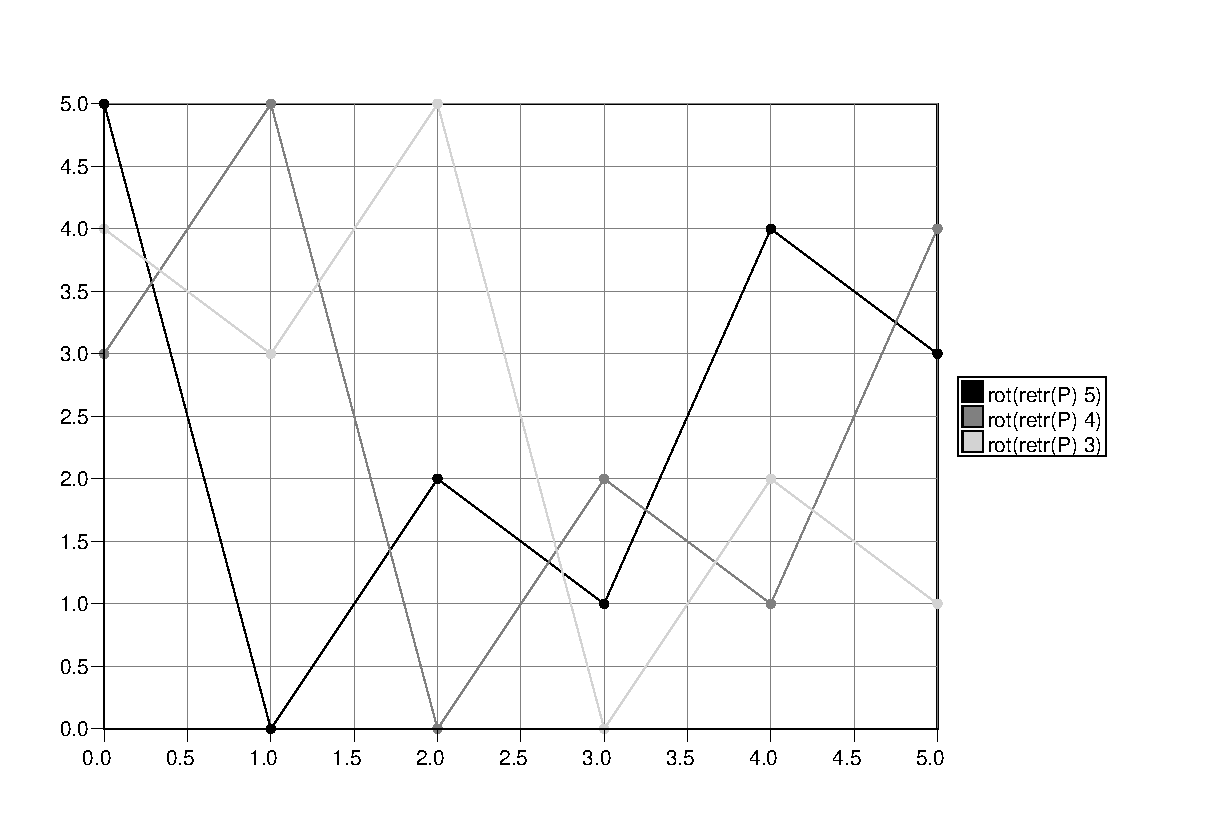
\includegraphics[scale=.44]{output-countersubject}
    \label{fig:output-contra-sujeito-fugato}
  }
  \caption{Software output for \eng{fugato} contour operations}
  \label{fig:output-fugato}
\end{figure}

\begin{figure}[!p]
  \centering
  \subfloat[4 fragments composed by rotation and expansion of an
  original contour]{
    \includegraphics[scale=1]{notas-curtas-madeiras}
    \label{fig:notas-curtas-madeiras}
  }

  \subfloat[original]{
    \includegraphics[scale=.75]{c-534120}
    \label{fig:rot-0}
  }
  \subfloat[rot 2]{
    \includegraphics[scale=.75]{c-412053}
    \label{fig:rot-2}
  }
  \subfloat[rot 3]{
    \includegraphics[scale=.75]{c-120534}
    \label{fig:rot-3}
  }
  \subfloat[retr(rot 3)]{
    \includegraphics[scale=.75]{c-435021}
    \label{fig:rot-3-retr}
  }
  \caption{Rotation and expansion}
  \label{fig:rotacao-expansao}
\end{figure}

%%% Local Variables: 
%%% mode: latex
%%% TeX-master: "contour-composition"
%%% End: 